\chapter{Разработка}
\section{Рендеринг}
Прежде чем приступать к созданию генератора, был необходим шейдер для отрисовки моделей. Этот шейдер должен поддерживать цветные вершины и плоское освещение, то есть такое освещение, при котором освещение вычисляется не для каждой отдельной вершины, а для целых полигонов. Такое освещение применяется в стиле low-poly для создания стилизованного изображения. 

Для демонстрационных целей в работе был использован шейдер, взятый из блога Hextant Studios. Результирующий плагин будет независим от конкретного шейдера, и в нём будет реализована поддержка отдельных материалов для листьев и ствола.

\section{Генерация листьев}
Разработка была начата с генератора круглой листвы. Для этого были изучены руководства по моделированию в стиле low-poly, чтобы максимально приблизить программную реализацию генератора к тому, как моделирует человек.

Генерация листьев проходит в несколько шагов:
\begin{enumerate}
\item Генерируется модель икосаэдра радиусом в одну единицу. У икосаэдра 12 вершин с координатами 
(\texttt{\(0, \pm\Phi, \pm1\)}), 
(\texttt{\(\pm1, 0, \pm\Phi\)}), 
(\texttt{\(\pm\Phi, \pm1, 0\)}) и 20 треугольных граней.\cite{IcosahedronMath}
Векторы вершин нормализуются, чтобы привести радиус фигуры к единице. Также фигура поворачивается на случайный угол.
 
\begin{lstlisting}
private const float PHI = 1.61803399f;

private void GenerateIcosahedron(float width,
    float height)
{
    var vectors = new Vector3[] {
        new Vector3(-1f, PHI, 0f),
        new Vector3(1f, PHI, 0f),
        new Vector3(-1f, -PHI, 0f),
        new Vector3(1f, -PHI, 0f),

        new Vector3(0f, -1f, PHI),
        new Vector3(0f, 1f, PHI),
        new Vector3(0f, -1f, -PHI),
        new Vector3(0f, 1f, -PHI),

        new Vector3(PHI, 0f, -1f),
        new Vector3(PHI, 0f, 1f),
        new Vector3(-PHI, 0f, -1f),
        new Vector3(-PHI, 0f, 1f)
    };

    var rotation = Random.rotation;
    foreach (Vector3 v in vectors) 
        AddVertex(rotation * v.normalized, color);

    // 5 faces around point 0
    AddTriangle(0, 11, 5);
    AddTriangle(0, 5, 1);
    AddTriangle(0, 1, 7);
    AddTriangle(0, 7, 10);
    AddTriangle(0, 10, 11);

    // 5 adjacent faces 
    AddTriangle(1, 5, 9);
    AddTriangle(5, 11, 4);
    AddTriangle(11, 10, 2);
    AddTriangle(10, 7, 6);
    AddTriangle(7, 1, 8);

    // 5 faces around point 3
    AddTriangle(3, 9, 4);
    AddTriangle(3, 4, 2);
    AddTriangle(3, 2, 6);
    AddTriangle(3, 6, 8);
    AddTriangle(3, 8, 9);

    // 5 adjacent faces 
    AddTriangle(4, 9, 5);
    AddTriangle(2, 4, 11);
    AddTriangle(6, 2, 10);
    AddTriangle(8, 6, 7);
    AddTriangle(9, 8, 1);
}
\end{lstlisting}

\item Для увеличения количества граней применяется алгоритм подразделения\cite{subdivision}, позволяющий создать приближённый к сфере многогранник путём разделения каждой грани на четыре и последующего смещения новых вершин на поверхность описанной сферы.
 
\begin{figure}[h]
    \centering
    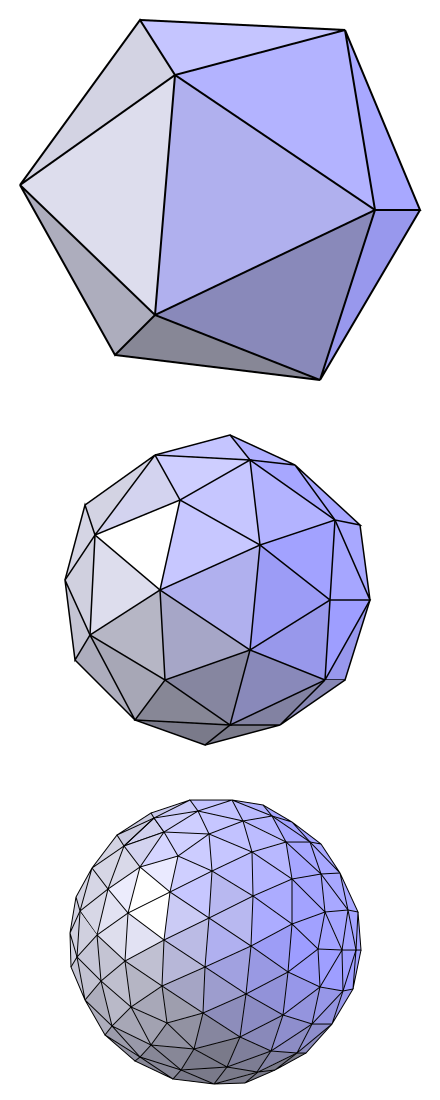
\includegraphics[height=0.5\textwidth, angle=90]{subdivision}
    \caption{Пример двукратного подразделения икосаэдра. Автор - Simon Fuhrmann, Wikimedia}
\end{figure}
 
Метод FindOrCreateMiddle находит вершину, находящуюся в середине отрезка между вершинами с заданными индексами, либо создаёт её, если её не существует.
\begin{lstlisting}
private int FindOrCreateMiddle(int aIndex, int bIndex)
{
    Vector3 a = vertices[aIndex];
    Vector3 b = vertices[bIndex];
    Vector3 middle = Vector3.Lerp(a, b, 0.5f)
        .normalized;

    int index = vertices.IndexOf(middle);
    if (index > -1) return index;

    return AddVertex(middle, color);
}

private void Subdivide()
{
    int n = triangles.Count;
    for (int i = 0; i < n; i += 3)
    {
        int a = FindOrCreateMiddle(triangles[i], 
            triangles[i + 1]);
        int b = FindOrCreateMiddle(triangles[i + 1], 
            triangles[i + 2]);
        int c = FindOrCreateMiddle(triangles[i + 2], 
            triangles[i]);

        AddTriangle(c, triangles[i], a);
        AddTriangle(a, triangles[i + 1], b);
        AddTriangle(b, triangles[i + 2], c);
        AddTriangle(a, b, c);
    }

    triangles.RemoveRange(0, n);
}
\end{lstlisting}

\item Фигура растягивается для достижения заданной ширины и высоты. Для каждой вершины вычисляется радиус (то есть длина вектора) по следующей формуле:

\begin{equation}
    r = lerp\left(width, height, \frac{\left|y_{v}\right|}{|v|}\right),
\end{equation}

где $lerp$ - функция линейной интерполяции, 

$width$ и $height$ - заданные ширина и высота листвы,

$v$ - вектор, задающий вершину.

\begin{lstlisting}
private void AdjustRadius()
{
    for (int i = 0; i < vertices.Count; i++)
    {
        Vector3 v = vertices[i];
        float radius = Mathf.Lerp(width, height, 
            Mathf.Abs(v.y) / v.magnitude);
        vertices[i] = v * radius;
    }
}
\end{lstlisting}

\item Наконец, вершины случайным образом смещаются для придания листве более натурального вида. Однако если две вершины поменяются местами, то геометрия листвы будет нарушена. Следовательно, для каждой вершины необходимо найти максимальный допустимый радиус смещения, при котором многогранник сохранит выпуклость.

Для нахождения максимально допустимого смещения используется следующая формула:

\begin{equation}
    maxshift_{i} = \frac{\displaystyle\min_{j = 0}^n(|V_{i} - N^{i}_{j}|)}{3}, 
\end{equation}
где $V$ - множество всех вершин, 

$N^{i}$ - множество соседей текущей вершины, 

$n$ - общее число соседей.

Полученное значение умножается на случайное значение от 0 до 1 и случайный единичный вектор, чтобы получить итоговое смещение для этой вершины.

\begin{lstlisting}
private IEnumerable<int> FindNeighbors(int k)
{
    for (int i = 0; i < triangles.Count; i += 3)
    {
        if (triangles[i] != k &&
            triangles[i + 1] != k &&
            triangles[i + 2] != k) continue;

        for (int j = i; j < i + 3; j++)
        {
            int other = triangles[j];
            if (other != k) yield return other;
        }
    }
}

private void DisplaceVertices()
{
    for (int i = 0; i < vertices.Count; i++)
    {
        float minDistance = float.MaxValue;

        Vector3 v = vertices[i];
        foreach (int j in FindNeighbors(i))
        {
            Vector3 neighbor = vertices[j];
            float distance = 
                Vector3.Distance(v, neighbor);
            if (distance < minDistance) 
                minDistance = distance;
        }

        float magnitude = 
            Random.value * (minDistance / 3);
        Vector3 displacement = 
            Random.insideUnitSphere * magnitude;

        vertices[i] = v + displacement;
    }
}
\end{lstlisting}
\end{enumerate}

\begin{figure}[h]
    \centering
    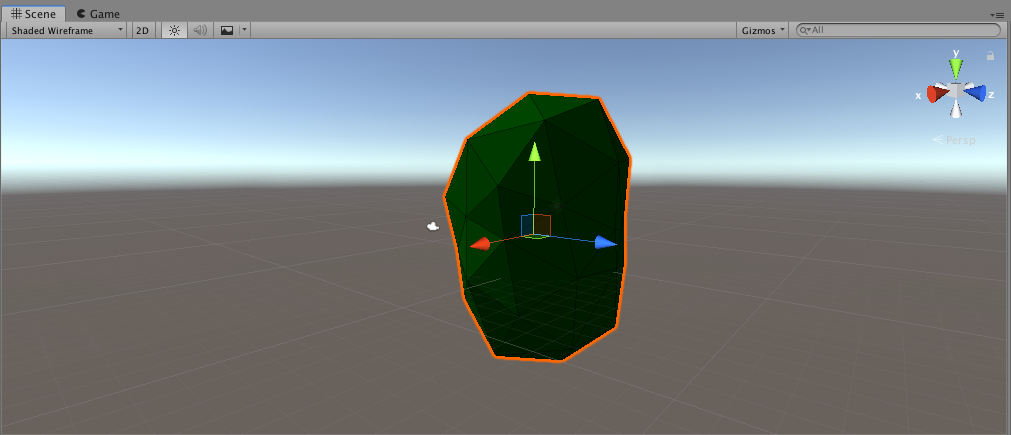
\includegraphics[height=0.4\textwidth]{foliage1}
    \caption{Процедурно сгенерированная листва.}
\end{figure}

\section{Генерация ствола}
На первых этапах разработки генератора стволов был рассмотрен схожий проект\cite{hassank} на Github, посвящённый анимации роста процедурно генерируемых деревьев. Этот проект был заброшен на ранней стадии разработки, но алгоритм генерации ствола, используемый в нём, оказался полезен в данной работе; он был доработан и усовершенствован.

Ствол представляет собой конус, разделённый на ярусы. Каждый ярус случайным образом поворачивается, задавая изгибы ствола. На конце ствола с помощью вышеописанного алгоритма генерируется крона, выделенная в отдельный игровой объект.

На стволе также могут генерироваться ветви. С определённой вероятностью происходит выбор грани на текущем уровне, из которого может вырасти ветвь. Ветви не могут расти слишком низко или слишком высоко. Также они не генерируются сразу; вместо этого создаётся объект генератора ветви и помещается в список, который будет обработан в последнюю очередь. Такое решение было принято для того, чтобы не нарушать порядок вершин, использованных в стволе. 

\begin{lstlisting}
public override void GenerateMesh()
{
    float radius = baseRadius;
    var rotation = Quaternion.identity;
    Vector3 pos = Vector3.zero;

    //Bottom of the tree
    AddRing(pos, 
        baseRadius * BASE_THICKNESS_MULTIPLIER, 
        rotation, barkColor);
    for (int i = 0; i < numSides - 2; i++) 
        AddTriangle(0, i + 1, i + 2);

    //Determine whether this tree is a stump
    bool isStump = stumpChance > 0 
        && URandom.value <= stumpChance;

    //Calculate actual height, which is lower 
    //than expected in case of a stump
    int actualHeight = isStump 
        ? URandom.Range(2, expectedHeight / 2) 
        : expectedHeight;

    for (int i = 0; i < actualHeight; i++)
    {
        radius = Mathf.Lerp(baseRadius, 0, 
            (float)i / expectedHeight);

        // Randomizing the branch angle
        float xRotation = (URandom.value - 0.5f) 
            * twisting;
        float zRotation = (URandom.value - 0.5f) 
            * twisting;
        rotation = Quaternion.Euler(xRotation, 0f, 
            zRotation);

        var shift = new Vector3(URandom.value - 0.5f, 
            0, URandom.value - 0.5f);
        pos += (rotation * Vector3.up + shift) * 
            tree.Scale;

        AddRing(pos, radius, rotation, barkColor);
        ConnectRings();

        //Attempt to sprout a branch
        float trunkPosition = (float)i / expectedHeight;
        if (trunkPosition >= 0.5 && trunkPosition <= 0.8)
        {
            if (URandom.value < 0.5f) 
                AddBranchGenerator();
        }
    }

    if (isStump) AddStumpTop(pos, radius, rotation);
    else
    {
        var capPos = pos + rotation * Vector3.up;
        AddBranchCap(capPos, barkColor);
        AddFoliage(rotation, capPos);
    }

    foreach (var g in branchGenerators) 
        g.GenerateMesh();

    PersistMesh();
}
\end{lstlisting}

Кроме того, с определённой вероятностью дерево может оказаться пнём. В таком случае оно будет обрублено в случайном месте. На срубе будет видна древесина и обломки коры.
\begin{lstlisting}
private void AddStumpTop(Vector3 topPos, float radius, 
    Quaternion rotation)
{
    int outerStartIndex = vertices.Count - numSides;
    AssertHelper.NotNegative(outerStartIndex);

    //Add the inner ring
    AddRing(topPos, radius * STUMP_INNER_RING_RADIUS, 
        rotation, barkColor);

    var direction = rotation * Vector3.up;
    int innerStartIndex = vertices.Count - numSides;

    for (int i = 0; i < numSides; i++) 
        AddSplinter(outerStartIndex, direction, i);

    //Fill the top of the stump
    AddRing(topPos, radius * STUMP_INNER_RING_RADIUS, 
        rotation, woodColor);
    int first = vertices.Count - numSides;
    for (int i = first; i < vertices.Count - 2; i++) 
        AddTriangle(i + 2, i + 1, first);
}
\end{lstlisting}


Метод AddBranchGenerator() пытается добавить на текущий уровень генератор ветви. Для этого выбирается случайная грань, из которой будет расти ветвь. Исходя из того, что ветви не растут вниз, для генерации ветви нормаль выбранной грани должна иметь положительную компоненту по вертикальной оси. Если это условие не выполняется, то генератор ветви не создаётся.
\begin{lstlisting}
private void AddBranchGenerator()
{
    int ringStartIndex = vertices.Count - 2 * numSides;
    int faceIndex = Random.Range(0, numSides - 1);

    //Find the normal of the face
    int i = ringStartIndex + faceIndex;
    int j = (faceIndex < numSides - 1) ? i + 1 : ringStartIndex;

    Vector3 normal = MeshHelper.Normal(
        vertices[i + numSides],
        vertices[j + numSides],
        vertices[i]
    );

    //Only generate if not facing down
    if (normal.y > 0)
    {
        //Find the center of the face
        Vector3 l = Vector3.Lerp(vertices[i], vertices[i + numSides], 0.5f);
        Vector3 r = Vector3.Lerp(vertices[j], vertices[j + numSides], 0.5f);
        Vector3 center = Vector3.Lerp(l, r, 0.5f);
        float radius = (l - r).magnitude / 2;

        var generator = new BranchGenerator(tree, mesh, this, center, normal, radius);
        branchGenerators.Add(generator);
    }
}
\end{lstlisting}

\section{Разработка расширения для редактора}
Для плагина было запланировано реализовать возможность генерации различных типов листвы - круглой, плоской и хвои. Однако у разных типов листьев могут быть разные параметры. Для удобной настройки в редакторе должны отображаться только те параметры, которые относятся к выбранному типу листвы. Чтобы решить эту задачу, было создано расширение для редактора.



\newpage
